\documentclass[12pt, a4paper, openany]{report}
\def\VersionRapport{1.0}
\usepackage[utf8]{inputenc} % un package
\usepackage[T1]{fontenc}      % un second package
\usepackage[francais]{babel}  % un troisième package
\usepackage{layout}
\usepackage[top=2.7cm, bottom=2.5cm, left=3.5cm, right=3cm]{geometry}
\usepackage{setspace}
\frenchbsetup{StandardLists=true} % à inclure si on utilise \usepackage[french]{babel}
%\usepackage{enumitem}
\usepackage[shortlabels]{enumitem}
\usepackage{amssymb}
\usepackage{color}
\usepackage{listings}
\definecolor{dkgreen}{rgb}{0,0.6,0}
\definecolor{gray}{rgb}{0.5,0.5,0.5}
\definecolor{mauve}{rgb}{0.58,0,0.82}
\definecolor{rougecerise}{rgb}{0.73,0.043,0.043}
\lstset{frame=tb,
  language=Matlab,
  aboveskip=3mm,
  belowskip=3mm,
  showstringspaces=false,
  columns=flexible,
  basicstyle={\small\ttfamily},
  keywordstyle=\color{blue},
  commentstyle=\color{dkgreen},
  stringstyle=\color{mauve},
  breaklines=true,
  breakatwhitespace=true,
  tabsize=3,
  breaklines=true,
  morekeywords={matlab2tikz},
  morekeywords=[2]{1}, 
  keywordstyle=[2]{\color{black}},
  identifierstyle=\color{black},
  numbers=left,
  numberstyle={\tiny \color{black}},
  numbersep=9pt, 
  emph=[1]{for,end,break},
  emphstyle=[1]\color{red}
}
\usepackage{multirow} % pour les tableaux
\usepackage[table]{xcolor} % pour les tableaux
\usepackage{verbatim}
%\usepackage{subcaption}
\usepackage{graphicx}
\usepackage{moreverb}
\usepackage{url}
\usepackage{pst-all}
\usepackage{eso-pic,graphicx}
\usepackage{caption} 
\usepackage[colorlinks=true,urlcolor=blue,linkcolor=red]{hyperref}
\usepackage{array}
\usepackage[toc,page]{appendix}
\usepackage[off]{auto-pst-pdf}
\usepackage{hyperref} % pour le sommaire table des matières
\AddThinSpaceBeforeFootnotes % à insérer si on utilise \usepackage[french]{babel}
\FrenchFootnotes % à insérer si on utilise \usepackage[french]{babel}
\usepackage{fancyhdr}
\pagestyle{headings}
\usepackage{pifont}  %pour les puces
\usepackage{amsmath,amsfonts,amssymb} %pour les puces
\usepackage{subfig}
\usepackage{verbatim} % pour le code en annexe 
%%%%%%%colones 
\newcolumntype{R}[1]{>{\raggedleft\arraybackslash }b{#1}}
\newcolumntype{L}[1]{>{\raggedright\arraybackslash }b{#1}}
\newcolumntype{C}[1]{>{\centering\arraybackslash }b{#1}}
%%%%%%% 
\renewcommand{\appendixpagename}{Annexes}
\renewcommand{\appendixtocname}{Annexes}
\title{Theme: Compte Rendu Commande des Systèmes Linéaires à Temps Discret}
\author{NAIMI \bsc{Nabil} \\ KHERBICHE \bsc{Ali}}
\date{2018-2019}
%new
\newcommand{\HRule}{\rule{\linewidth}{0.5mm}}

\begin{document}

%\selectlanguage{francais}
\pagenumbering{arabic} 
\makeatletter
\begin{titlepage}
\begin{sffamily}
\begin{center}
    % Upper part of the page. The '~' is needed because \\
    % only works if a paragraph has started.
    
\includegraphics[scale=0.5]{Logo_UT3.jpg}~\\[1cm]
    \textsc{\LARGE M1 ISTR-RODECO  }\\[1cm]
    \textsc{\Large Compte Rendu Commande des Systèmes Linéaires à Temps Discret}\\[1cm]
    % Title
    \HRule \\[0.4cm] % saut de ligne
    { \huge  \textsc {Commande échantillonnée d'un Procédé $\ll$ Bille sur Rail $\gg$ par Retour d'état avec Observateur \\[0.4cm] }}

    \HRule \\[1cm]   % sous de ligne 
    
\includegraphics[scale=0.1]{logomaster.jpg}
    \\[1cm]
    % Author and supervisor
    \begin{minipage}{0.4\textwidth}
      \begin{flushleft} \large
         \textsc{\emph {Fait par:} \\KHERBICHE Ali\\ NAIMI Nabil}  
          \newline
          Promotion 2018-2019 \\
      \end{flushleft}
    \end{minipage}
    \begin{minipage}{0.4\textwidth}
      \begin{flushright} \large
        %%\emph{Tuteur et}
        \emph{Tuteurs:\\} \textsc{M Frédéric GOUAISBAUT\\M Soheib FERGANI}
      \end{flushright}
    \end{minipage}
    \vfill
    % Bottom of the page
    {\large Avril 2018}
  \end{center}
  \end{sffamily}                
  \end{titlepage}  
\makeatother
   
%*********************** somaire **************
\renewcommand{\contentsname}{Sommaire}
\tableofcontents
%*********************** listes des figures **************
\listoffigures
%*********************** listes des tableaux **************
%\listoftables

\chapter*{\textsc{Introduction}}
\addcontentsline{toc}{chapter}{\textsc{Introduction}}

	\paragraph{} Le but de cette manipulation est de'implémenter une loi de commande par retour de sortie sur un procédé complexe. Elle comporte trois parties : 
	
	\begin{itemize} [label=\ding{70},font=\small \color{black}]
  	\item la première partie concerne l'analyse sommaire du procédé selon qu'il est commandé et observé en contenu ou bien de manière échantillonnée par calculateur;\\ 
    \item dans un deuxième temps, on synthétise une commande par retour d'état assurant un asservissement de la sortie avec une précision suffisante et un régime transitoire compatible avec le domaine de fonctionnement normal du système; \\
    \item un estimateur permettant de reconstruire les états du système inaccessibles à la mesure est ensuite mis en place; la loi de commande précédente est alors modifiée de façon à effectuer le retour sur les états éstimés, puis elle est implémentée sur le procédé.\\
	\end{itemize}
	
	\begin{center}
	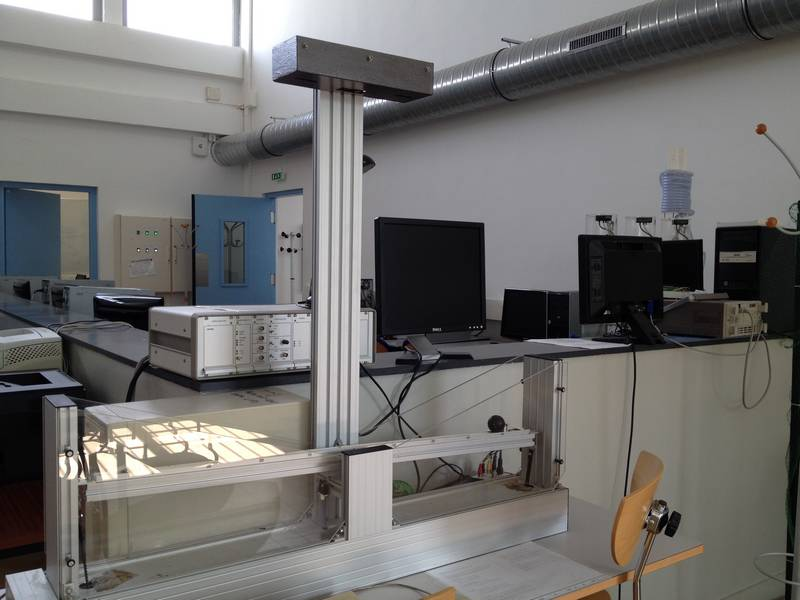
\includegraphics[scale=0.4]{bille.jpg}
	\captionof{figure}{\textit{Platine <<bille sur rail>> \\}}
	\label{fig1} 
	\end{center}	

\break
\chapter{\textsc{Représentation d'état du procédé }}

	\begin{center}
	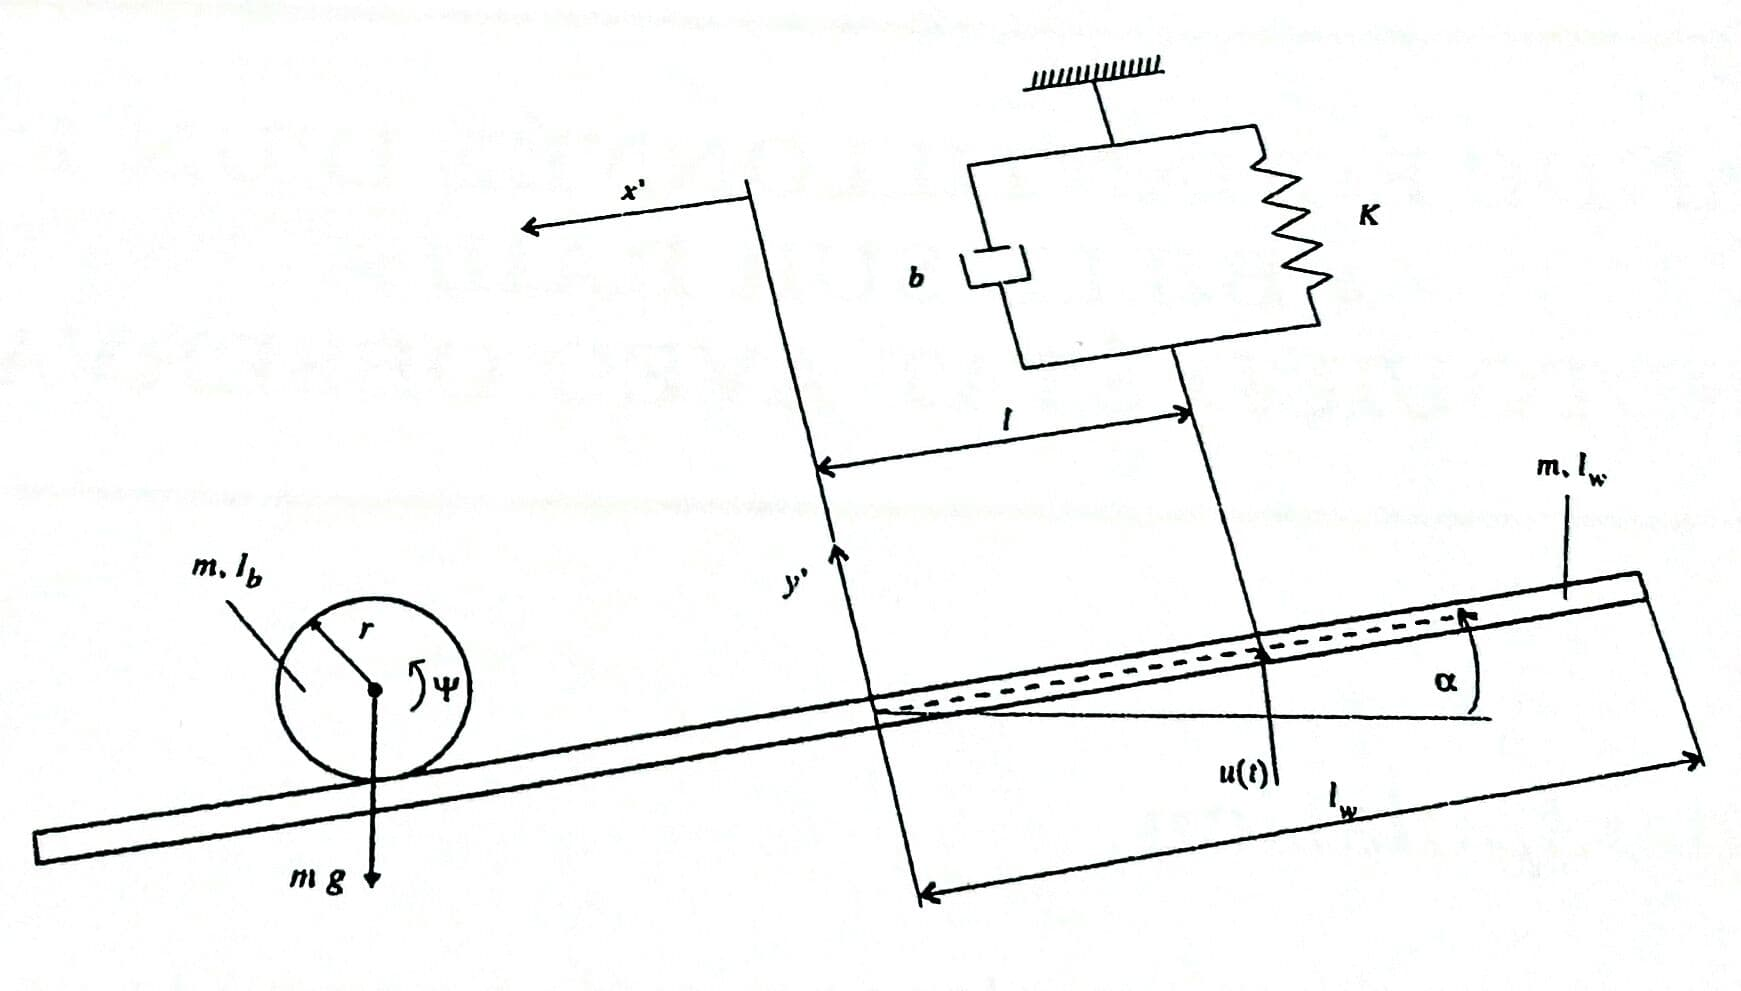
\includegraphics[scale=0.2]{procede.jpg}
	\captionof{figure}{\textit{représentation schématique de la platine <<bille sur rail>> \\}}
	\label{fig2} 
	\end{center}	
L'étude mécanique a conduit à la représentation d'état suivante:\\

	\begin{center}
		$ \dot{x}(t)=Ax(t)+Bu(t)$ \\[0.25 cm]
		$y(t)=Cx(t) $

	\end{center}
Avec $x(t)=[x_1(t) \hspace{1 mm} x_2(t) \hspace{1 mm} x_3(t) \hspace{1 mm} x_4(t)]^T, \hspace{1 mm} y(t) = [y_1(t), \hspace{1 mm} y_2(t)]^T $, et :\\

$A = \begin{pmatrix}
	0 & 1 & 0 & 0 \\
	A_{21} & 0 & A_{23} & A_{24} \\
	0 & 0 & 0 & 1 \\
	A_{41} & 0 & A_{43} & A_{44}  
\end{pmatrix} \hspace{0.25 cm} B = \begin{pmatrix}
	0 \\
	B_2 \\
	0 \\
	B_4  
\end{pmatrix} \hspace{0.25 cm} C = \begin{pmatrix}
	1 & 0 & 0 & 0 \\
	0 & 0 & 1 & 0 
\end{pmatrix}$

Les quatre composants du vecteur d'état $x(t)$ sont donc, respectivement et avec les conventions de signes définies plus haut:

\begin{itemize} [label=\ding{70},font=\small \color{black}]
  	\item  $x_1(t)$ : la position de la bille sur le rail (en $m$).
    \item  $x_2(t)$ : la vitesse de la bille sur le rail (en $m.s^{-1}$).
    \item  $x_3(t)$ : l'angle entre le rail et l'horizontale (en $rad$).
    \item  $x_4(t)$ : la vitesse  angulaire (en $rad.s^{-1}$).
	\end{itemize}

Pour la bille en acier, les coefficients des matrices dynamique et de commande des représentations précédentes sont les suivants:\\
$A_{21}= -0.3421 s^{-2} \hspace{2 cm} A_{23}= 6.5982 s^{-2} \hspace{2 cm} A_{24}= 0.0310 s^{-2} $\\
$ A_{21}= 18.8975 s^{-2} \hspace{2 cm} A_{23}= -0.3404 s^{-2} \hspace{2 cm} A_{44}= -1.7130 s^{-2} $\\
$ B_2 = -0.0633 kg^{-1} \hspace{2 cm} B_4 = 3.4960 kg^{-1}  $\\
\chapter{\textsc{Analyse du procédé en boucle ouverte}}
\section{\textsc{ Analyse du modèle à temps discret de l'ensemble (bloqueur d'ordre $0$, procédé en boucle ouverte) }}
\subsection{\textsc{La description sur les matrices d'état $ A_d,\hspace{1mm}B_d $ et $ C_d $ }}

De la représentation d'état on trouve :
	\begin{center}
		$ \dot{x}(t)=Ax(t)+Bu(t)$\\
 		$ \Longrightarrow  x(t) = e^{At} x(0) + \overset{t}{\underset{0}{ \int }} e^{ A(t-h)} Bu(h) dh $\\
 		et $y(t)=Cx(t) $
	\end{center}
Soit $T_e$ la période d'échantillonnage, avec: $t \in [kT_e,(k+1)T_e]$, et $u(t)=cste=u$:\\

	\begin{center}
		$ x[(k+1)T_e] = e^{AT_e} x(kT_e) + \overset{T_e}{\underset{0}{ \int }} e^{ A(T_e-h)} Bu(h) dh $\\
 		$ x[(k+1)T_e] = e^{AT_e} x(kT_e) +  \overset{t}{\underset{0}{ \int }} e^{ A(T_e-h)}dh Bu $ \\[0.5 cm]
 		\end{center}
 		
 		Du coup: \\
 		\begin{center}
 		$ x[(k+1)T_e] = e^{AT_e} x(kT_e) + [A^{-1}(e^{AT_e}-I_d)] Bu $ si $A$ est inversible.\\[0.25 cm]
 		et $y(kT_e)=Cx(kT_e)$
	\end{center}
Par identification avec les relations suivantes:\\ 
	\begin{center}
		$ x[(k+1)T_e] = A_d x(kT_e) + B_d u(kT_e) $\\
 		et $y(kT_e)=C_d x(kT_e)$\\
	\end{center}	
On trouve: 
	\begin{center}
		$ A_d = e^{AT_e} $\\
		$ B_d = A^{-1}(e^{AT_e}-I_d) $ si $A$ est inversible.\\  
 		$ C_d = C $
	\end{center}

	
	
%\input{chap2.tex}
%\input{chap3.tex}
%\input{conclusion.tex}
%\input{annexes.tex}
%*********************** Bibliographie ************ 
\bibliographystyle{alpha}
\bibliography{biblio}  



\end{document}